\documentclass[UTF8,zihao=-4]{ctexart}
\usepackage[a4paper,margin=22mm]{geometry}
\usepackage{amsmath,tikz}
\newcommand{\ans}[2]{\par\medskip\noindent\textbf{#1}\quad #2\par}
\begin{document}
\section*{电路理论基础｜A 卷参考答案}
\ans{1．C}{$I_l=\sqrt3 I_\Delta=4\sqrt3$ A。}
\ans{2．B}{互易性要求两个方向的传递阻抗相等，即 $Z_{12}=Z_{21}$。}
\ans{3．错}{串联谐振时 $X_L=X_C$，两端电压相量等大反向，和为零；各元件的电压仍可很高。}
\ans{4．对}{半周期反对称使前后半周期的直流贡献抵消。第 $n$ 次谐波平移半周期后乘以 $(-1)^n$，故只能保留奇数次。原卷公式中的负号应读作 $u(t+T/2)=-u(t)$。}
\ans{5．2 mH，14 mH}{顺反接分别为 $L_1+L_2\pm2M$，两式相减得 $4M=8$ mH，取平均得自感之和。}
\ans{6．100 安匝，400 A/m}{$NI=200\times0.5$；均匀磁路中 $H=NI/l=100/0.25$。}
\ans{7．周期 4 s，平均值 1.5 V，有效值 3 V}{占空比为 $1/4$，故平均值为 $6/4$ V，有效值为 $\sqrt{6^2/4}$ V。}
\begin{tikzpicture}[x=.85cm,y=.34cm]
\draw[->](0,0)--(8.6,0) node[right]{$t$/s};\draw[->](0,0)--(0,7) node[above]{$u$/V};
\draw[thick,blue](0,0)--(0,6)--(1,6)--(1,0)--(4,0)--(4,6)--(5,6)--(5,0)--(8,0);
\draw[dashed](0,1.5)--(8,1.5)node[right]{1.5 V};\node[left]at(0,6){6};\foreach \x in {0,1,4,5,8}\node[below]at(\x,0){\x};
\end{tikzpicture}
\ans{8．串联谐振}{$R=2/0.1=20\,\Omega$，$Q=f_0/\Delta f=10$。由 $Q=2\pi f_0L/R$ 得 $L=31.83$ mH，再由 $C=1/[(2\pi f_0)^2L]$ 得 $C=0.796\,\mu$F。}
\ans{9．258 W}{两次开路试验分别给出矩阵的第一、二列：
$Z=\begin{bmatrix}14/2&12/3\\8/2&18/3\end{bmatrix}=\begin{bmatrix}7&4\\4&6\end{bmatrix}\,\Omega$。代入电流 $(2,5)$ A 得电压 $(34,38)$ V，总吸收功率 $34\times2+38\times5=258$ W。}
\ans{10．RC 放电}{电容电压连续，初值 12 V；终态无电流，终值 4 V。$\tau=RC=8$ ms。以秒计时，$u_C=4+8e^{-t/0.008}$ V，$i_C=C\,du_C/dt=-2e^{-t/0.008}$ mA。令 $u_C=6$ 得 $t=8\ln4=11.09$ ms；电容释放 $\tfrac12 C(12^2-6^2)=108\,\mu$J。}
\newpage
\section*{电路理论基础｜B 卷参考答案}
\ans{1．C}{$\underline U_{AB}=\underline U_{AN}-\underline U_{BN}$；正序下比 A 相相电压超前 $30^\circ$。}
\ans{2．B}{$f_0=1/(2\pi\sqrt{LC})$，电容变为四倍，频率减半。}
\ans{3．错}{不同频率的交叉项平均为零，总有效值为 $\sqrt{\sum I_n^2}$。}
\ans{4．对}{前级的输出变量就是后级的输入变量，依次代入得 $T=T_1T_2$。}
\ans{5．500 Ω，200 Ω}{静态电阻 $U/I=2/0.004$；小信号电阻 $du/di=1/0.005$。}
\ans{6．72 Ω，0.5 A}{原边等效阻抗 $3^2\times8=72\,\Omega$；副边电压为 $12/3=4$ V，故电流为 $4/8=0.5$ A。}
\ans{7．二表法}{图中星号标同名端，左侧电源，右侧负载。电流线圈串入 A、C 线，电压线圈分别测 $u_{AB}$、$u_{CB}$。由 $i_A+i_B+i_C=0$ 得总有功功率 $P=W_1+W_2$，按读数符号相加。}
\begin{tikzpicture}[x=1cm,y=.78cm]
\foreach \y/\s in {2/A,0/B,-2/C}{\node[left] at(0,\y){\s};}
\foreach \y/\n in {2/1,-2/2}{\draw(0,\y)--(1,\y) node[midway,above]{*};\node[draw,minimum width=1.5cm] (i\n) at(1.8,\y){$W_\n$ 电流};\draw(i\n.east)--(6,\y);\fill(4,\y)circle(2pt);\node[draw] (v\n) at(4,\y/2){$W_\n$ 电压};\draw(4,\y)--(v\n);\draw(v\n)--(4,0);\node[right]at(4,\y*.83){*};}
\draw(0,0)--(6,0);\fill(4,0)circle(2pt);
\end{tikzpicture}
\ans{8．三相功率}{三角形相电压为 150 V，$|Z|=15\,\Omega$，故相电流 10 A，线电流 $10\sqrt3$ A。$P=3I_\Delta^2 R=3600$ W，$Q=3I_\Delta^2 X=2700$ var（感性）。}
\ans{9．输入电阻 6 Ω}{串联、并联两级的矩阵相乘：
$T=\begin{bmatrix}1&4\\0&1\end{bmatrix}\begin{bmatrix}1&0\\0.25&1\end{bmatrix}=\begin{bmatrix}2&4\\0.25&1\end{bmatrix}$，其中 $B$ 用 Ω、$C$ 用 S。输出并联支路等效 $4\parallel4=2\,\Omega$，再串联 4 Ω 即得。}
\ans{10．RL 脉冲响应}{$u_s=8[\varepsilon(t)-\varepsilon(t-1)]$ V，$\tau=L/R=0.5$ s。零时刻前 $i=0$；$0\le t<1$ 时 $i=2(1-e^{-2t})$ A。$i(1)=1.729$ A，储能 $Li(1)^2/2=2.991$ J。之后 $i=2(1-e^{-2})e^{-2(t-1)}$ A。由 $di/dt=(u_s-Ri)/L$，左右斜率分别为 $+0.541$、$-3.459$ A/s。}
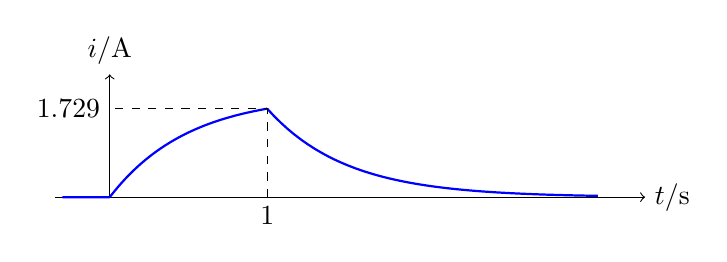
\begin{tikzpicture}[x=2cm,y=.65cm]
\draw[->](-.35,0)--(3.4,0)node[right]{$t$/s};\draw[->](0,0)--(0,2.4)node[above]{$i$/A};
\draw[blue,thick](-.3,0)--(0,0) plot[domain=0:1,samples=40](\x,{2*(1-exp(-2*\x))}) plot[domain=1:3.1,samples=50](\x,{2*(1-exp(-2))*exp(-2*(\x-1))});
\draw[dashed](1,0)node[below]{1}--(1,1.729)--(0,1.729)node[left]{1.729};
\end{tikzpicture}
\newpage
\section*{电路理论基础｜C 卷参考答案}
\ans{1．B}{直流与谐波分别贡献均方值，总有效值为 $\sqrt{3^2+4^2}=5$ V。}
\ans{2．A}{负实部决定振幅衰减，共轭虚部产生振荡，对应欠阻尼。}
\ans{3．错}{只将独立源置零，保留受控源。在端口施加测试源，以测试电压与流入网络的电流之比求等效电阻。}
\ans{4．对}{正弦磁通下 $E=4.44 fN\Phi_m$，频率和磁通幅值固定时，感应电压与匝数成正比。}
\ans{5．$(6-j8)\,\Omega$，10 Ω}{复负载取共轭匹配；纯电阻取 $|Z_s|=\sqrt{6^2+8^2}$。}
\ans{6．0.5，19 mH}{$k=M/\sqrt{L_1L_2}=3/6$；顺接等效电感为 $4+9+2\times3=19$ mH。}
\ans{7．工作点 (3 V，3 mA)}{取 V、mA 为单位，负载线为 $i=6-u$。元件第二段斜率为 2 mA/V，故 $i=1+2(u-2)$；联立可得交点，且 $2<3<4$，落在该段内。}
\begin{tikzpicture}[x=.85cm,y=.42cm]
\draw[->](0,0)--(7,0)node[right]{$u$/V};\draw[->](0,0)--(0,7)node[above]{$i$/mA};
\draw[blue,thick](0,6)node[left]{6}--(6,0)node[below]{6};\draw[thick](0,0)--(2,1)--(4,5)node[right]{元件特性};
\fill(3,3)circle(2pt);\draw[dashed](3,0)node[below]{3}--(3,3)--(0,3)node[left]{3};
\end{tikzpicture}
\ans{8．线电流 8 A}{每相总阻抗 $9+j12$ Ω，模为 15 Ω，线电流等于相电流 $120/15=8$ A。线路总铜损 $3\times8^2\times1=192$ W，电源总有功功率 $3\times8^2\times9=1728$ W。}
\ans{9．输出有效值 $\sqrt{11.5}=3.391$ V}{电容端传递函数为 $H(j\omega)=1/(1+j\omega RC)$。基波幅值 $5/\sqrt2$ V，相位 $-45^\circ$；三次谐波幅值 $5/\sqrt{10}$ V，相位 $-\arctan3=-71.57^\circ$。直流仍为 2 V；两交流幅值先除以 $\sqrt2$ 再合成，总均方值 $4+25/4+25/20=11.5$。}
\ans{10．临界阻尼阶跃响应}{取秒为时间单位。换路后 $i'=8-4i-u_C$，$u_C'=4i$，初值均为零。消去电流得 $u_C''+4u_C'+4u_C=32$。特征方程 $(s+2)^2=0$ 有重根，故为临界阻尼。令 $u_C=8+(a+bt)e^{-2t}$，由 $u_C(0)=0$、$u_C'(0)=4i(0)=0$ 得 $a=-8,b=-16$。因此 $u_C=8[1-(1+2t)e^{-2t}]$ V，$i=u_C'/4=8te^{-2t}$ A。终值为 8 V、0 A，与电容在直流稳态开路一致。}
\end{document}
